\documentclass{beamer}
\usetheme{Boadilla}
\usepackage[utf8]{inputenc}
\usepackage[english]{babel}
\usepackage{blindtext}
\usepackage{hyperref}

\hypersetup{
    colorlinks=true,
    linkcolor=blue,
    filecolor=magenta,      
    urlcolor=cyan,
    pdftitle={hyperref one},
    bookmarks=true,
    pdfpagemode=FullScreen,
    }
    
\urlstyle{same}

\title{Winter Workshop}
\subtitle{Beamer Assignment}
\author{
    Rohan Yadav\\19MCMI07
}
\institute{SCIS, UOH}
\date{\today}

\begin{document}
    \begin{frame}
        \titlepage
    \end{frame}
    
    \begin{frame}
        \frametitle{Contents}
        \tableofcontents
    \end{frame}
    
    \section{Introduction}
    
    \begin{frame}
        \frametitle{John Von Neumann}
        \begin{columns}
            \column{0.5\textwidth}
                \begin{figure}
                    \centering
                    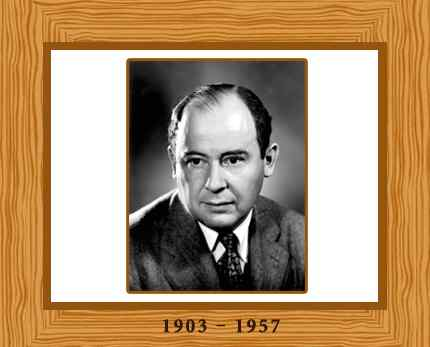
\includegraphics[scale=0.39]{res/images/john-von-neumann.jpg}
                    \caption{John Von Neumann}
                    \label{fig:neumann}
                \end{figure}
            \column{0.5\textwidth}
                \begin{itemize}
                    \item John von Neumann (December 28, 1903 – February 8, 1957) was a Hungarian-American mathematician, physicist, computer scientist, and polymath.
                    \item Von Neumann wrote 150 published papers in his life; 60 in pure mathematics, 20 in physics, and 60 in applied mathematics.
                    \item He has \hyperlink{contributed}{contributed} a lot to the computer science community.
                \end{itemize}
        \end{columns}
    \end{frame}

    \section{Major Work}
    \begin{frame}{Major Work:}
    \hypertarget{contributed} Figure \ref{fig:neumann} was a Hungarian mathematician who made important contributions to mathematics, physics, computer science, and the area of artificial life. He was born in Budapest, Hungary, on 28 December 1903.\\
    Theory of Games and Economic Behavior, published in 1944 \cite{game-theory} by Princeton University Press, is a book by mathematician John von Neumann and economist Oskar Morgenstern which is considered the groundbreaking text that created the interdisciplinary research field of game theory.
    \end{frame}

    \section{References}
    \begin{frame}\frametitle{References :}
        \bibliographystyle{plain}
        \bibliography{bib.bib}
    \end{frame}
    \begin{frame}
        \begin{center}
            \vfill
                {\Huge Thank you}
            \vfill
        \end{center}
    \end{frame}
\end{document}